\documentclass{article}
\usepackage[spanish]{babel}
\usepackage[utf8]{inputenc}
\usepackage{graphicx}
\graphicspath{ {./images/} }
\usepackage{hyperref}
\usepackage{subcaption}
\usepackage{geometry} % see geometry.pdf on how to lay out the page. There's lots.
\geometry{a4paper} % or letter or a5paper or ... etc
% \geometry{landscape} % rotated page geometry

% See the ``Article customise'' template for come common customisations


\author{Tomás Bacigalupo , Lucio Pagni}
\date{\today}
\author{Tomas Bacigalupo y Lucio Pagni}
\date{18/07/2020} % delete this line to display the current date

%%% BEGIN DOCUMENT
\begin{document}

% caratula
\begin{titlepage}
\centering
{
\includegraphics[width=1\textwidth]{./images/logoitba.png}\par}
\vspace{1cm}
{\scshape\Large Simulaci\'on de Sistemas \par}
\vspace{3cm}
{\scshape\Huge COVID-19\par}
\vspace{3cm}
{\itshape\Large Trabajo Pr\'actico Final \par}
\vfill
{\Large Autores: \par}
{\Large Tomas Bacigalupo, Lucio Pagni\par}
\vfill
{\Large \today \par}
\end{titlepage}
\clearpage

\listoffigures   % generate list of figures
\clearpage
\listoftables % generate list of tables    
 \clearpage

\tableofcontents
\clearpage

\section{Introducción}
Se trabajo durante la segunda mitad del cuatrimestre en un software de simulación de personas comprando en un supermercado. Nuestro trabajo en el desarrollo fue el de estructurar el proyecto y desarrollar el modulo de la caja que consta de atender clientes y encolarlos en la fila correcta. Por otro lado el trabajo de estructura nos llevo a tomar decisiones como desarrollos de pom.xml con sus respectivas dependencias en cada modulo y como tarea principal se implementaron todos los módulos a travez de un main que permitía mediante un archivo de configuración establecer las variables de la simulación. Y es en este momento donde comienza nuestro trabajo de desarrollo para esta entrega final, donde se mejoraron los tiempos de simulación mediante la mejora de nuestros dos módulos: Main y Caja

\section{Implementación}
En cuanto a la estructura, luego de varias idas y vueltas de los distintos grupos de trabajo se opto por una implementación simple de Interfaces e Implementaciones, con el objetivo de programar contra interfaces como se puede ver en la figura \ref{grafico}



\section{Simulaciones}
texto

\section{Resultados}
texto

\section{Concluciones}
texto

\section{Apéndice}
texto

\clearpage
\section{Figuras}
\begin{figure}[h]
\begin{center}
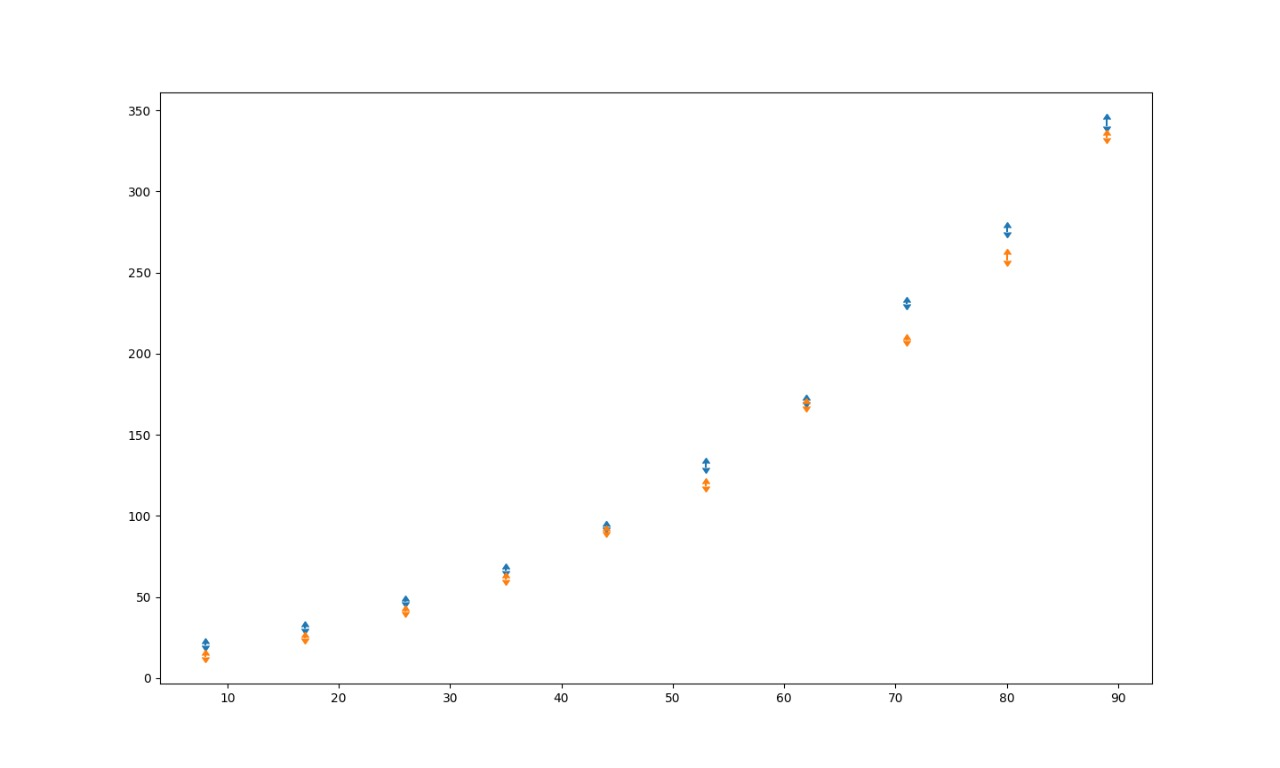
\includegraphics[width=4in]{./images/inputVsOutput.jpeg}
\caption{Ejemplo aca va la descripcion }
\label{grafico}
\end{center}
\end{figure}
\clearpage

\end{document}